\documentclass[14pt]{beamer}

\usetheme[secheader]{Boadilla}

% Presento style file
\usepackage{tikz}
\usetikzlibrary{tikzmark,fit,shapes.geometric}

% Information
\title{Courbes planes paramétrées}
\subtitle{Partie 1}
\author{Y. Carissan}
%\institute{www.ratulsaha.com}
\date{2020}

\AtBeginSection[]{\begin{frame}{Plan}\tableofcontents[currentsection,hideothersubsections]\end{frame}}

\begin{document}

% Title page
\begin{frame}{}
\maketitle
\end{frame}

\begin{frame}{Plan}
        \tableofcontents[hideallsubsections]
\end{frame}

\section{Courbes planes en paramétrage cartésien}
\subsection{Définition}
\begin{frame}
        \begin{alertblock}{Définition~: Courbe plane paramétrée}
        On appelle courbe plane paramétrée un ensemble de points du plan, noté $(r)$,
tel qu'il existe une fonction vectorielle:
                \begin{align*}
                \begin{array}{lll}
                        \vec{F}: & I &\to \mathbb{R}^2\\
                        & t &\mapsto \overrightarrow{OM}(t)
                \end{array}
                \end{align*}
avec $I$ un intervalle de $\mathbb{R}$ et $M$ un point de $(r)$.
\end{alertblock}
\end{frame}

\subsection{Remarques}
\begin{frame}{}
        \begin{block}{Remarques}
                \begin{enumerate}
                        \item $\vec{F}$ est appelée représentation paramétrique de $(r)$.
                        \item Si on note $x(t)$ et $y(t)$ les coordonnées cartésiennes du point $M(t)$, on a:
                \begin{align*}
                \begin{array}{lll}
                        \vec{F}: & I &\to \mathbb{R}^2\\
                        & t &\mapsto \left\{\begin{array}{r}x(t)\\y(t)\end{array}\right.
                \end{array}
                \end{align*}
        \item Le réel $t$ est un paramètre. Il n'apparaitra pas sur le dessin.
                \end{enumerate}
        \end{block}
\end{frame}

\subsection{Exemples}
\begin{frame}{}
        \begin{exampleblock}{Exemple 1}
                \begin{enumerate}
                        \item Si on pose $x(t)=t$ et $y(t)=f(t)$ la courbe $\mathcal{C}$ qui représente
                                une fonction $f(x)$ a pour représentation paramétrique~:
                \begin{align*}
                \begin{array}{lll}
                        \vec{F}: & I &\to \mathbb{R}^2\\
                        & t &\mapsto \left\{\begin{array}{l}x(t)=t\\y(t)=f(t)\end{array}\right.
                \end{array}
                \end{align*}
                \end{enumerate}
        \end{exampleblock}
\end{frame}
\begin{frame}{}
        \begin{exampleblock}{Exemple 2}
                \begin{enumerate}
        \item Le cercle de centre $O$ et de rayon $1$ a pour équation cartésienne $x^2 + y^2 = 1$
                et pour représentation paramétrique~:
                \begin{align*}
                \begin{array}{lll}
                        \vec{F}: & \mathbb{R} &\to \mathbb{R}^2\\
                        & t &\mapsto \left\{\begin{array}{r}x(t)=\cos t\\y(t)=\sin t\end{array}\right.
                \end{array}
                \end{align*}
                \end{enumerate}
        \end{exampleblock}
\end{frame}

\section{Tangente en un point}
\subsection{Dérivabilité}
\subsubsection{Définition}
\begin{frame}
        \begin{alertblock}{Définition~: Dérivabilité}
                Soit $I$ un intervalle de $\mathbb{R}$.\\
                Soit 
                \begin{align*}
                        \begin{array}{lll}
                        \vec{F}: & \mathbb{R} &\to \mathbb{R}^2\\
                        & t &\mapsto \overrightarrow{OM}(t)
                \end{array}
                \end{align*}
                une représentation paramétrique.\\
                Soit $t_0\in I$.
                On dit que $\vec{F}$ est dérivable en $t_0$ lorsque:
                \begin{align*}
                        \lim_{t\to t_0}\frac{\vec{F}(t)-\vec{F}(t_0)}{t-t_0}
                \end{align*}
                existe et est finie.
        \end{alertblock}
\end{frame}

\subsubsection{Remarques}
\begin{frame}{}
        \begin{block}{Remarques}
                \begin{enumerate}
                        \item Lorsque la limite existe, on note~:
                \begin{align*}
                        \vec{F\;'}(t_0) & = \lim_{t\to t_0}\frac{\vec{F}(t)-\vec{F}(t_0)}{t-t_0}
                \end{align*}
        \item Si on pose $\vec{F}(t) = x(t) \vec{i} + y(t) \vec{j}$ alors
                $\vec{F\;'}(t)= x\;'(t) \vec{i} + y\;'(t) \vec{j}$
        \item Soit $p\in \mathbb{N}$, on a aussi~:
                \begin{align*}
                        \vec{F^{(p)}}(t)= x^{(p)}(t) \vec{i} + y^{(p)}(t) \vec{j}
                \end{align*}
        \item On dit que $M_0(t_0)$ est stationnaire si $\vec{F\;'}(t_0)=\vec{0}$
                \end{enumerate}
        \end{block}
\end{frame}

\subsubsection{Interprétation géométrique de $\vec{F\;'}(t_0)$}
\begin{frame}{Interprétation géométrique de $\vec{F\;'}(t_0)$}
        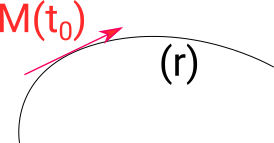
\includegraphics[width=0.4\textwidth]{images/tangente.png}\\
        Soit $(r)$ une courbe paramétrée par $\vec{F}$.\\
        Soit $M(t_0)$ un point de $(r)$.\\
        Si $\vec{F}$ est dérivable en $t_0$ et si $\vec{F\;'}(t)\ne\vec{0}$
        alors il existe une tangente à $(r)$ en $M$.\\
        Cette tangente est la droite qui passe par $M$ et qui est dirigée
        par le vecteur $\vec{F\;'}(t_0)$.
\end{frame}
\begin{frame}{Proposition importante}
        \begin{alertblock}{Définition à retenir}
                Soit $(r)$ une courbe paramétrée par $\vec{F}$.\\
                Soit $M_0(t_0)$ un point de (r).\\
                S'il existe $p\in\mathbb{N}$ tel que $\vec{F}^{(p)}\ne\vec{0}$,
                alors $(r)$ admet une tangente en $M_0$ dirigée par le premier
                vecteur dérivé non nul.
        \end{alertblock}
\end{frame}

\section{Exercice d'application}
\subsection{Énoncé}
\begin{frame}
        \begin{exampleblock}{Exercice d'application}
        Soit~:
        \begin{align*}
                \begin{array}{lll}
                        \vec{F}: & \mathbb{R} &\to \mathbb{R}^2\\
                        & t &\mapsto \left\{\begin{array}{l}x(t)=t^2\\y(t)=\cos t\end{array}\right.
                \end{array}
        \end{align*}
        Étudier la tangente en $t=0$.
        \end{exampleblock}
\end{frame}
\subsection{Résolution}

\begin{frame}{Résolution 1/2}
Pour $t=0$, on a le point $A(x(0);y(0)) = (0; 1)$.\\
        Au point A, on calcule la dérivée de $\vec{F}$~:
        \begin{align*}
                \vec{F\;'}(t) = \left(\begin{array}{cc}2t\\-\sin t\end{array}\right) \text{ donc }
                \vec{F\;'}(0) = \left(\begin{array}{cc}0\\0\end{array}\right)
        \end{align*}
        $\vec{F\;'}(0)=\vec{0}$ on calcule donc la dérivée seconde de $\vec{F}$ en $0$~:
        \begin{align*}
                \vec{F\;"}(t) = \left(\begin{array}{cc}2\\-\cos t\end{array}\right) \text{ donc }
                \vec{F\;"}(0) = \left(\begin{array}{cc}2\\-1\end{array}\right)
        \end{align*}
        $\vec{F\;"}(0)\ne\vec{0}$ est le premier vecteur dérivé non nul.
\end{frame}

\begin{frame}{Résolution 2/2}
        \begin{itemize}
                \item $\vec{F\;"}(0)\ne\vec{0}$, il dirige donc la tangente à la courbe en $A$.
                \item De plus, comme $\vec{F\;'}(0)=\vec{0}$, on note que A est un point stationnaire.
        \end{itemize}
\end{frame}

\section{Branches infinies}
\subsection{Asymptote et branches paraboliques}
\begin{frame}

        \begin{alertblock}{Définition: asymptote}
                $(r)$ admet en $t_0$ une asymptote d'équation
                $y=ax+b$ signifie~: "Lorsque $t$ tend $t_0$
                la courbe se rapproche de la droite $y=ax+b$
                sans jamais la couper."
        \end{alertblock}
        \begin{alertblock}{Définition: branche parabolique}
                $(r)$ admet en $t_0$ une branche parabolique
                de direction $y=ax$ signifie~: "Lorsque $t$
                tend vers $t_0$, la courbe s'éloigne de la droite
                $y=ax$ en prenant la forme d'une parabole."
        \end{alertblock}
\end{frame}
\subsection{Définition}
\begin{frame}
        \begin{alertblock}{Définition}
                Soit $(r)$ la courbe paramétrée par
                \begin{align*}
                \begin{array}{lll}
                        \vec{F}: & I &\to \mathbb{R}^2\\
                        & t &\mapsto \left\{\begin{array}{l}x(t)\\y(t)\end{array}\right.
                \end{array}
                \end{align*}
                Soit $t_0\in\mathbb{R}\cup\{-\infty\}\cup\{+\infty\}$.
                On dit que $(r)$ admet une branche infinie en $t_0$
                lorsque $x(t)$ ou $y(t)$ tendent vers l'infini
                quand $t$ tend vers $t_0$.
        \end{alertblock}
\end{frame}

\subsubsection{Seul $y(t)$ tend vers l'infini si $t \to t_0$}
\begin{frame}{Seul $y(t)\to\infty$ si $t \to t_0$}
        \begin{alertblock}{Proposition}
                Soit $t_0\in\mathbb{R}\cup\{-\infty\}\cup\{+\infty\}$.\\
                Soit $c\in\mathbb{R}$.
                \begin{align*}
                        \text{Si } \lim_{t\to t_0}x(t)=c & \text{ et }\lim_{t\to t_0}y(t)=\pm\infty
                \end{align*}
                alors $x=c$ est asymptote à $(r)$ en $t_0$.
        \end{alertblock}
\end{frame}
\begin{frame}{Seul $y(t)\to\infty$ si $t \to t_0$}
        \begin{exampleblock}{Exemple $(r)$ paramétrée par}
        \begin{align*}
                \begin{array}{lll}
                        \vec{F}: & \mathbb{R} &\to \mathbb{R}^2\\
                        & t &\mapsto \left\{\begin{array}{l}\cos t\\-\frac{1}{(t-\frac{\pi}{4})^2}-2\end{array}\right.
                \end{array}
        \end{align*}
        \end{exampleblock}
        On a bien:
        \begin{align*}
                \lim_{t\to \frac{\pi}{4}}x(t)=\frac{\sqrt{2}}{2} & \text{ et }\lim_{t\to \frac{\pi}{4}}y(t)=-\infty
        \end{align*}
        $x=\frac{\sqrt{2}}{2}$ est donc asymptote à $(r)$ \textbf{lorsque $t$ est proche de $\frac{\pi}{4}$}.
\end{frame}

\begin{frame}{Seul $y(t)\to\infty$ si $t \to t_0$}
        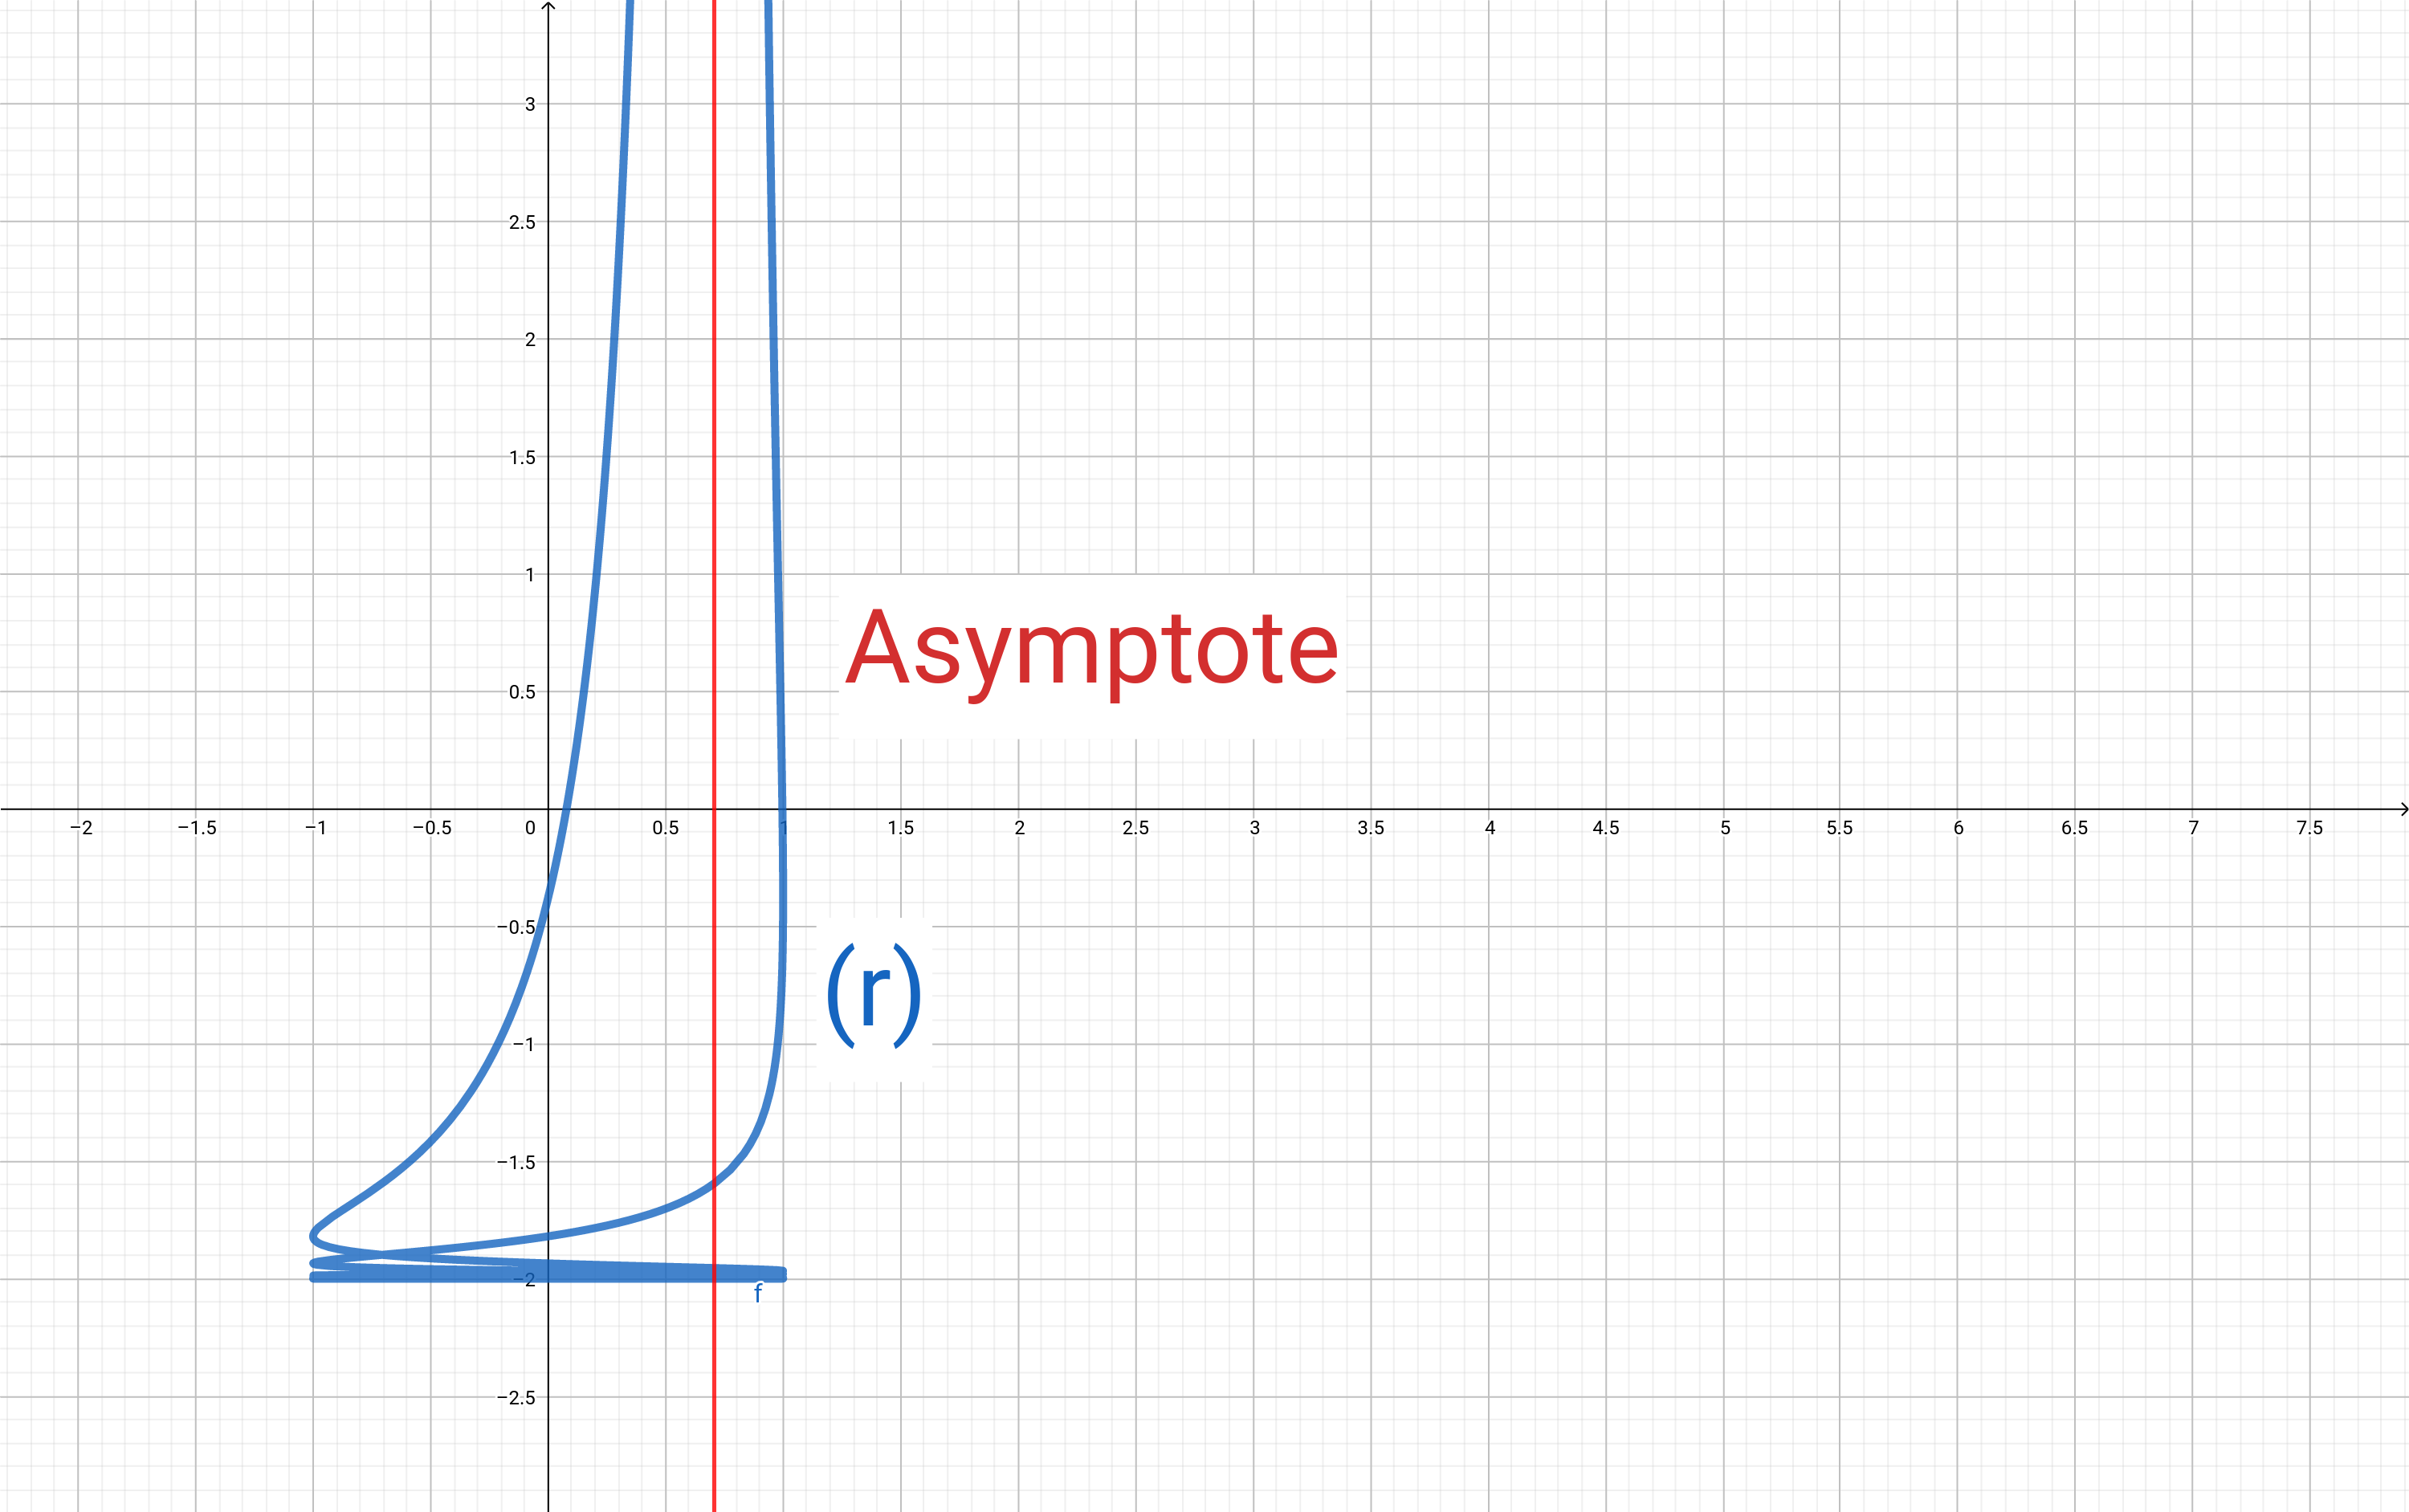
\includegraphics[height=0.8\textheight]{images/Asymptote_01.png}
\end{frame}

\subsubsection{Seul $x(t)$ tend vers l'infini si $t \to t_0$}
\begin{frame}{Seul $x(t)\to\infty$ si $t \to t_0$}
        \begin{alertblock}{Proposition}
                Soit $t_0\in\mathbb{R}\cup\{-\infty\}\cup\{+\infty\}$.\\
                Soit $c\in\mathbb{R}$.
                \begin{align*}
                        \text{Si } \lim_{t\to t_0}y(t)=c & \text{ et }\lim_{t\to t_0}x(t)=\pm\infty
                \end{align*}
                alors $y=c$ est asymptote à $(r)$ en $t_0$.
        \end{alertblock}
\end{frame}
\begin{frame}{Seul $x(t)\to\infty$ si $t \to t_0$}
        \begin{exampleblock}{Exemple $(r)$ paramétrée par}
        \begin{align*}
                \begin{array}{lll}
                        \vec{F}: & \mathbb{R} &\to \mathbb{R}^2\\
                        & t &\mapsto \left\{\begin{array}{l}\frac{1}{(t+\frac{\pi}{3})^2}+1\\\sin t\end{array}\right.
                \end{array}
        \end{align*}
        \end{exampleblock}
        On a bien:
        \begin{align*}
                \lim_{t\to -\frac{\pi}{3}}x(t)=+\infty & \text{ et }\lim_{t\to -\frac{\pi}{3}}y(t)=-\frac{\sqrt{3}}{2}
        \end{align*}
        $y=-\frac{\sqrt{3}}{2}$ est donc asymptote à $(r)$ \textbf{lorsque $t$ est proche de $-\frac{\pi}{3}$}.
\end{frame}

\begin{frame}{Seul $x(t)\to\infty$ si $t \to t_0$}
        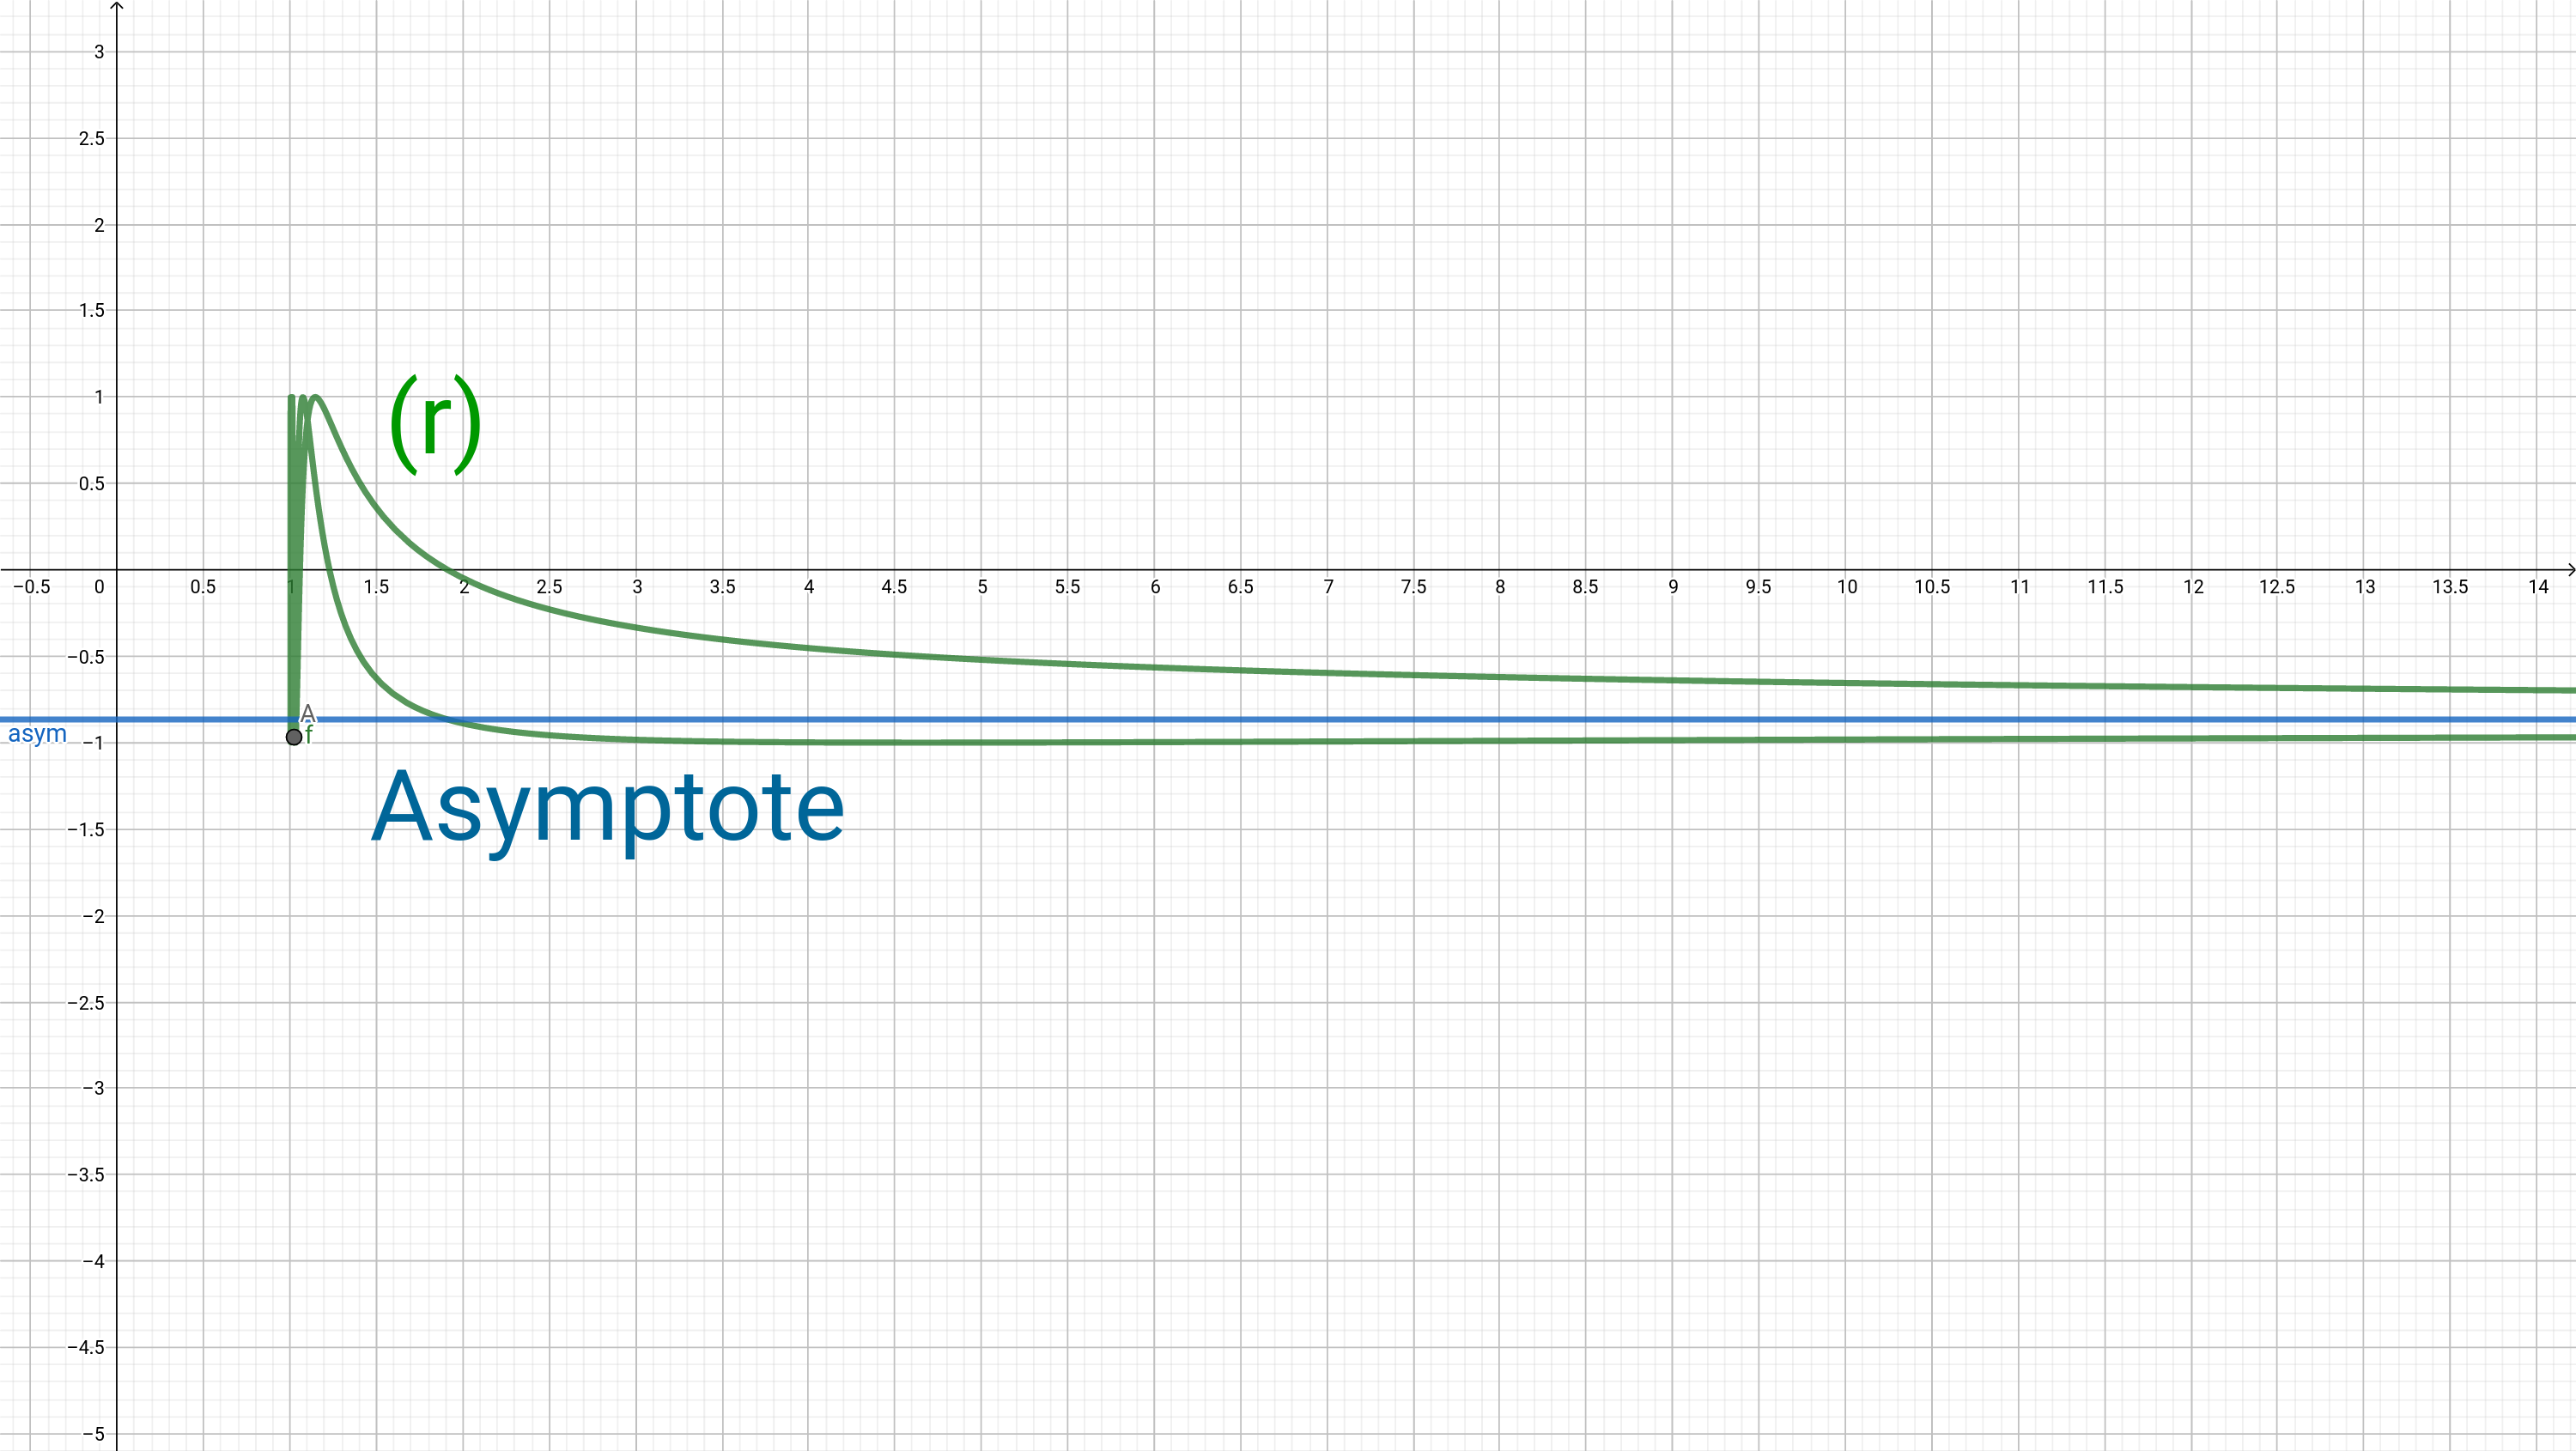
\includegraphics[height=0.8\textheight]{images/Asymptote_02.png}
\end{frame}

\subsubsection{$x(t)$ et $y(t)$ tendent vers l'infini si $t \to t_0$}
\begin{frame}{$x(t)$ et $y(t)$ tendent vers l'infini si $t \to t_0$}
        On suppose que~:
        \begin{align*}
                \left\{\begin{array}{l}
                        \lim_{t\to t_0} x(t) = \pm\infty\\
                        \lim_{t\to t_0} y(t) = \pm\infty
                \end{array}\right.
        \end{align*}
        Pour déterminer les asymptotes et le branches paraboliques, on devra calculer~:
        \begin{align*}
                \lim_{t\to t_0}\frac{y(t)}{x(t)}
        \end{align*}
        On étudiera $3$ cas, selon la valeur de cette limite: $0, \pm\infty, a$ avec $a\in\mathbb{R}$.
\end{frame}

\begin{frame}{Cas n°1}
        \begin{align*}
                \lim_{t\to t_0}\frac{y(t)}{x(t)}=0
        \end{align*}
        La courbe admet une branche parabolique d'axe $(Ox)$ en $t_0$.
        \begin{exampleblock}{Exemple: la fonction racine carrée}
                \begin{minipage}[b]{5cm}
                La fonction racine carrée admet une branche parabolique d'axe (Ox) en $0$.
                \end{minipage}
                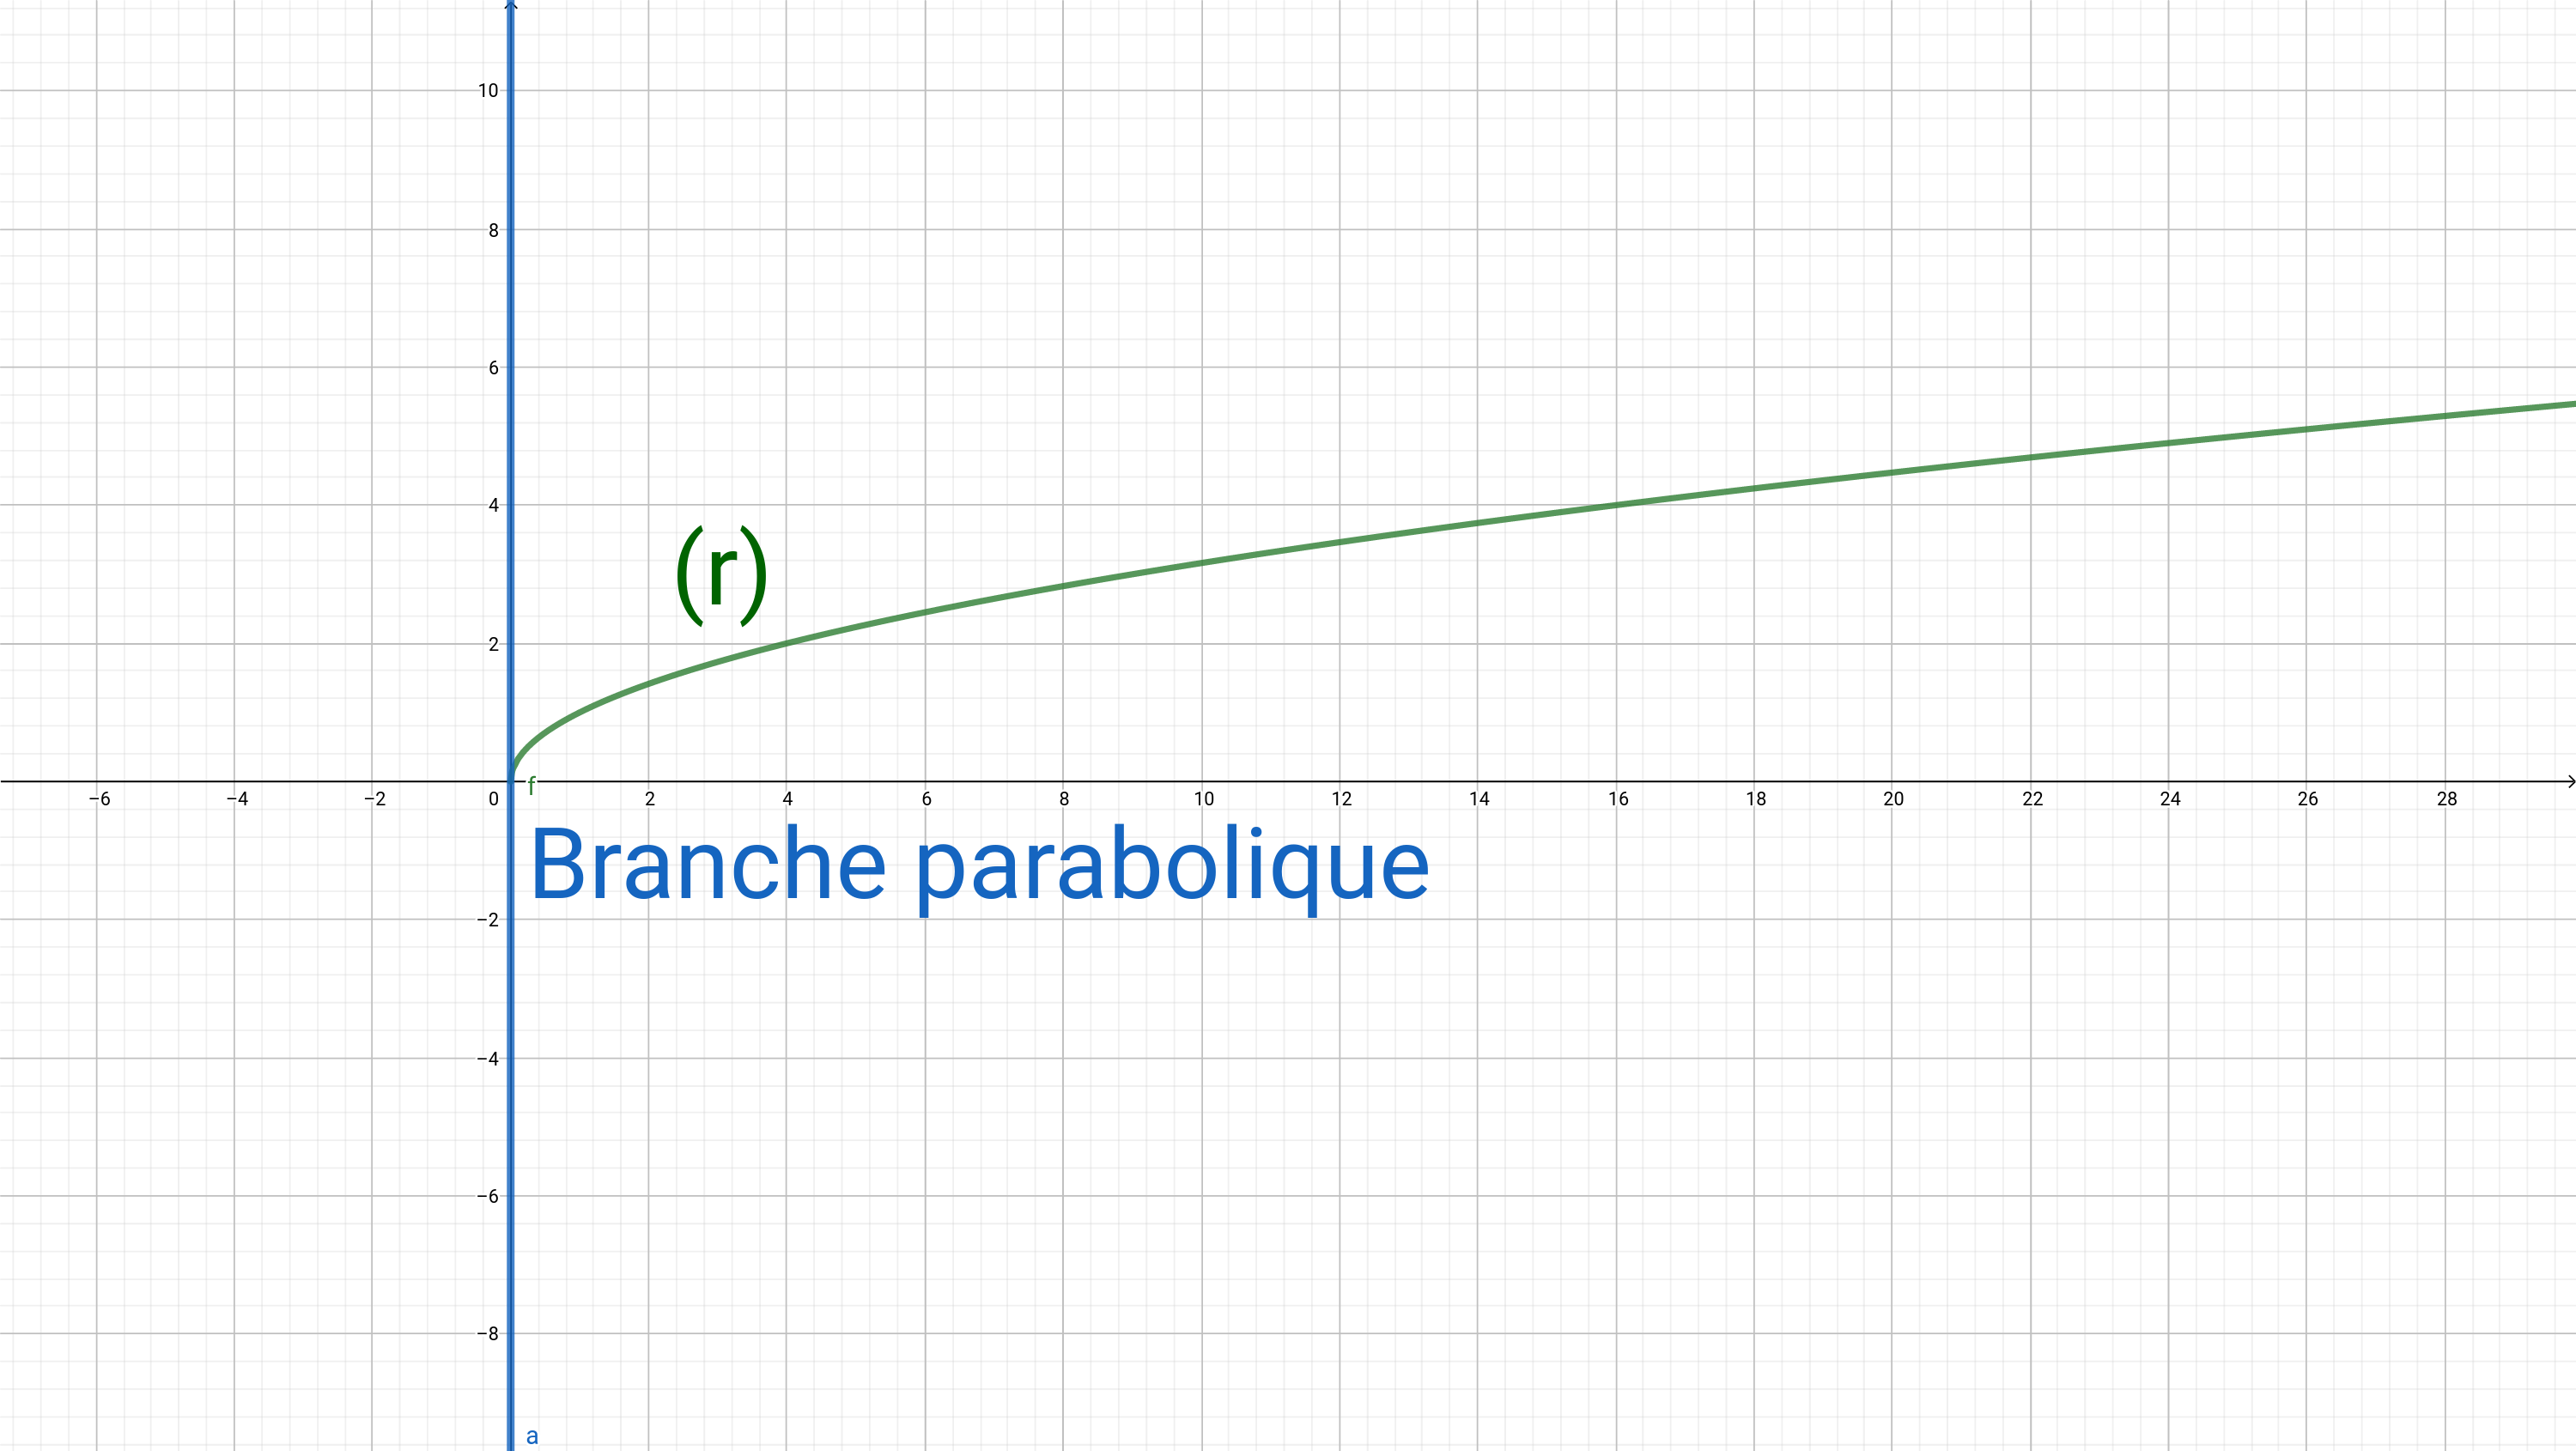
\includegraphics[height=3cm]{images/racine.png}
        \end{exampleblock}
\end{frame}

\begin{frame}{Cas n°2}
        \begin{align*}
                \lim_{t\to t_0}\frac{y(t)}{x(t)}=\pm\infty
        \end{align*}
        La courbe admet une branche parabolique d'axe $(Oy)$ en $t_0$.
        \begin{exampleblock}{Exemple: la fonction carré}
                \begin{minipage}[b]{5cm}
                La fonction carré admet une branche parabolique d'axe (Oy) en $0$.
                \end{minipage}
                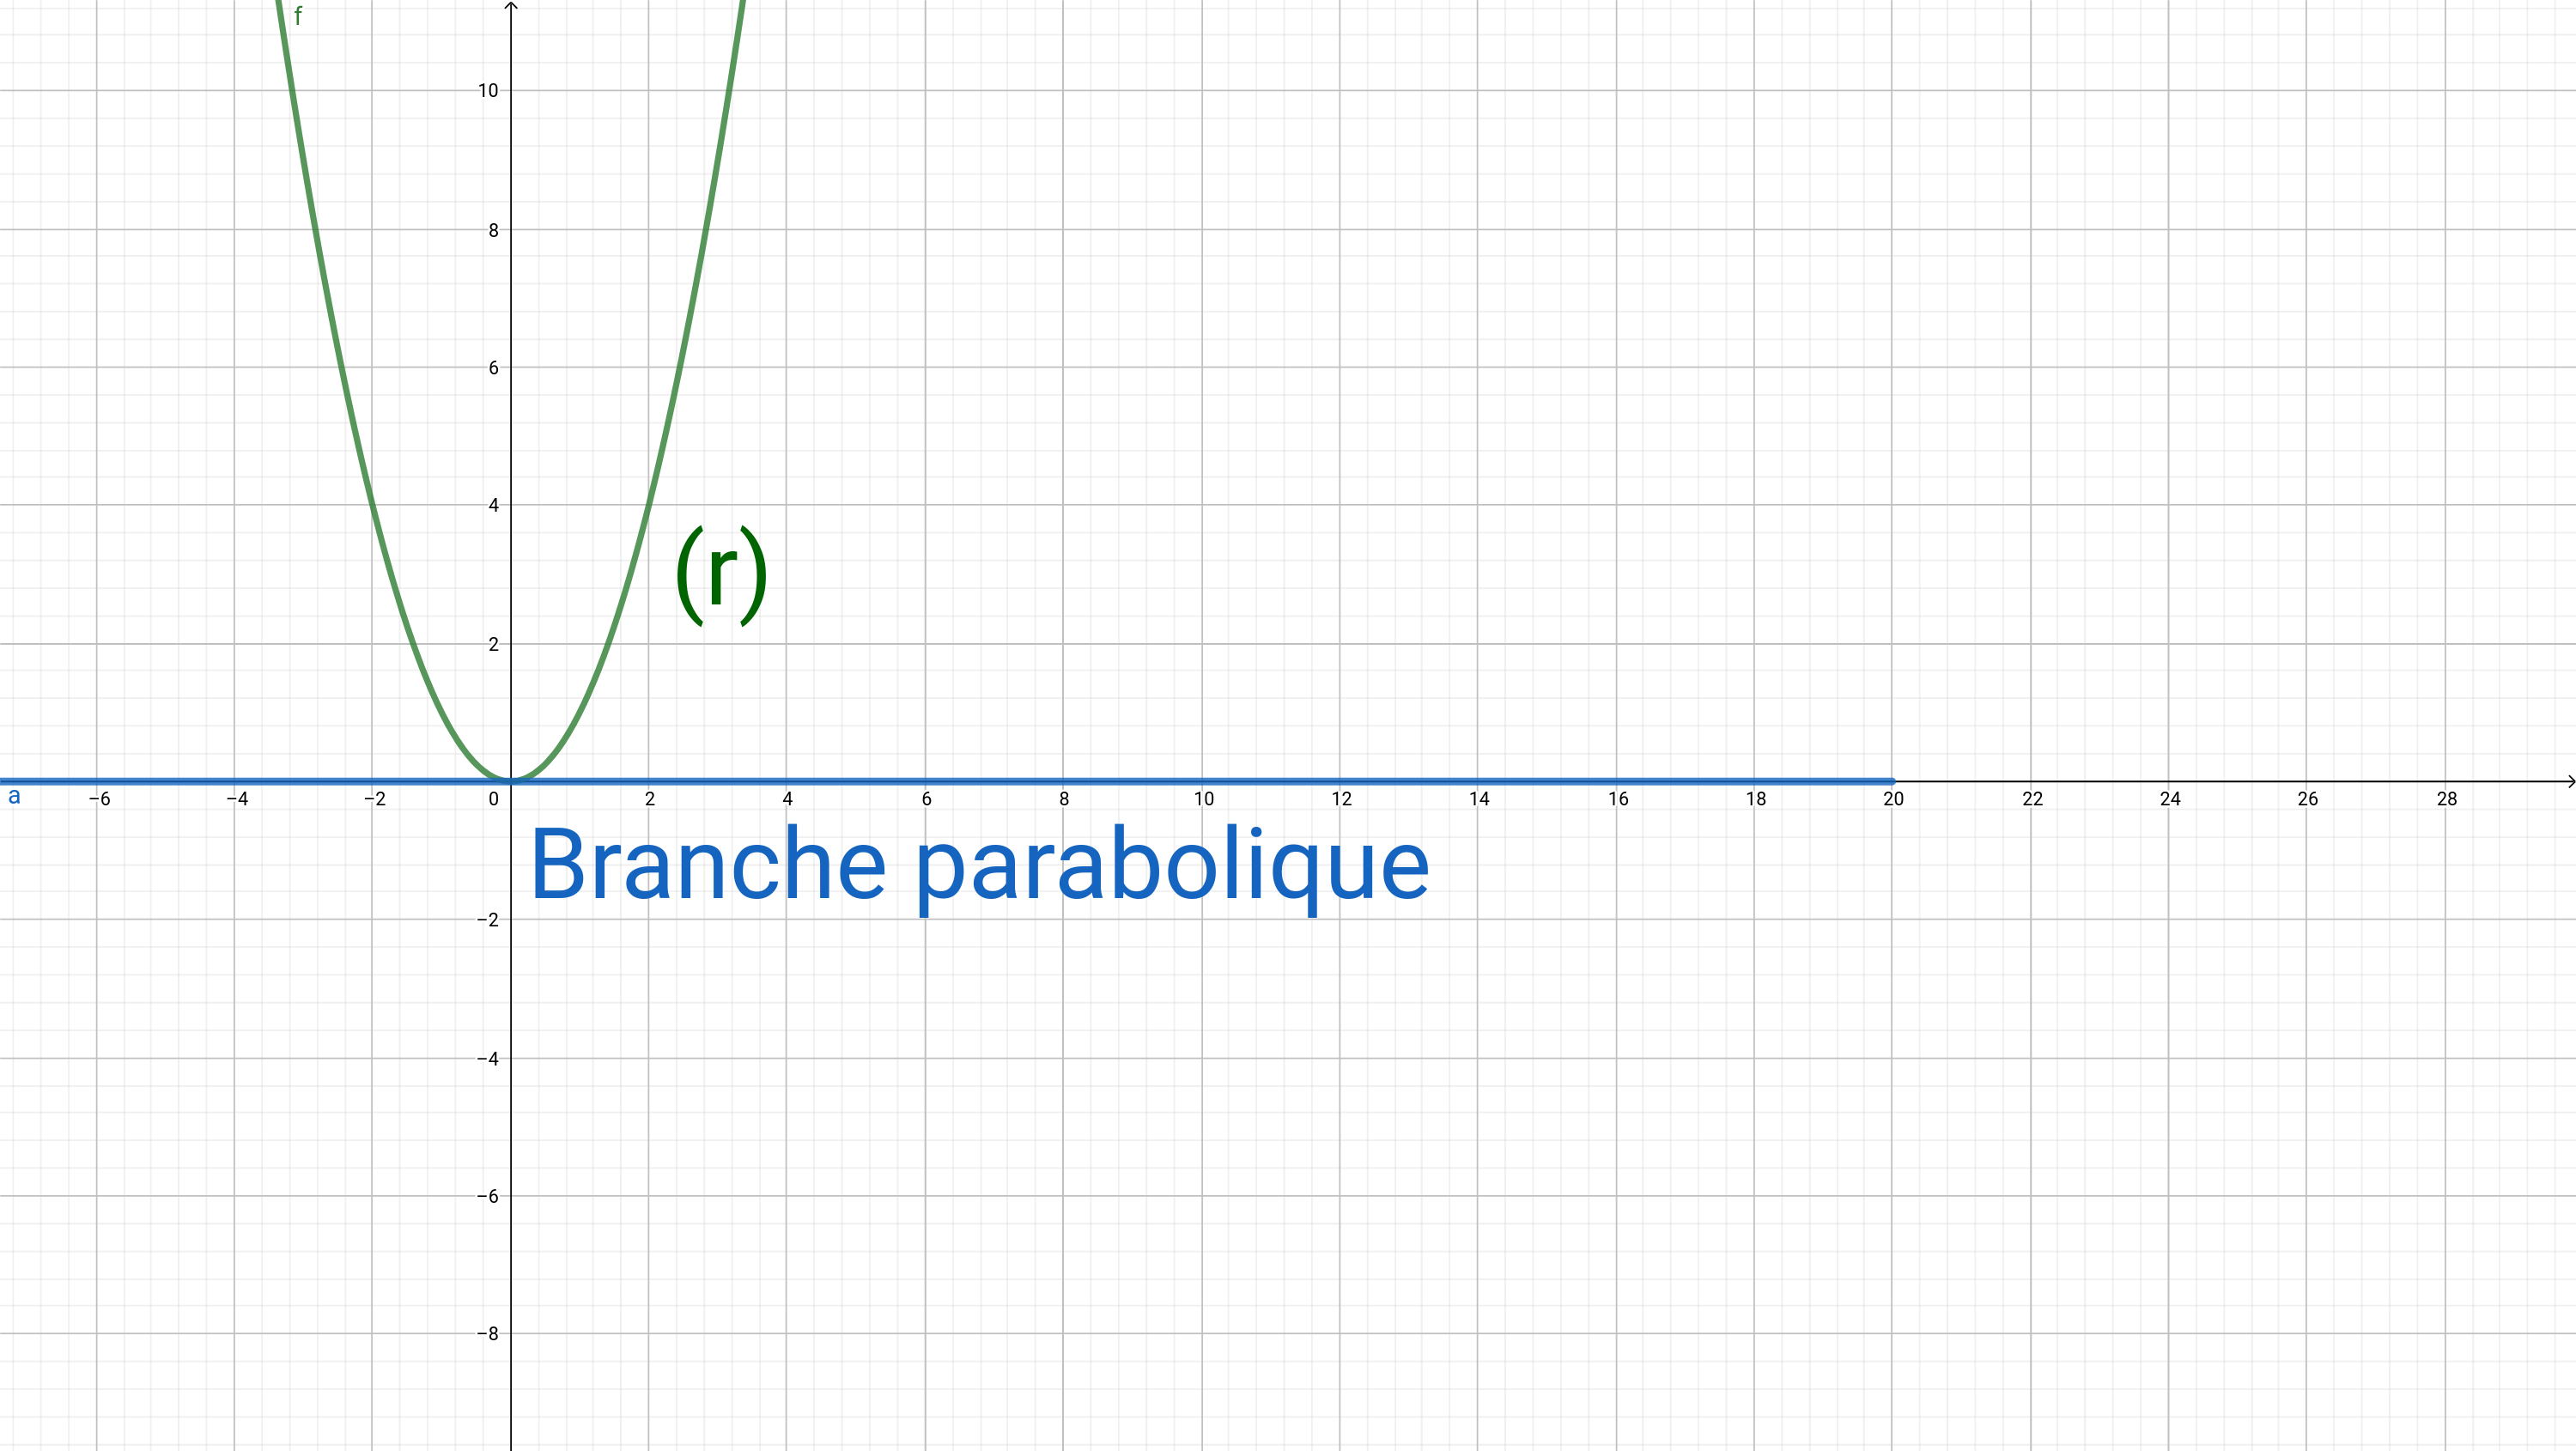
\includegraphics[height=3cm]{images/carre.png}
        \end{exampleblock}
\end{frame}

\begin{frame}{Cas n°3}
        \begin{align*}
                \lim_{t\to t_0}\frac{y(t)}{x(t)}=a\text{ avec }a\in\mathbb{R}
        \end{align*}
        C'est le cas le plus complexe.
        On calcule $\lim_{t\to t_0}\left[y(t)-ax(t)\right]$
        et on a 2 cas~:
        \begin{itemize}
                \item[$\alpha$] $\lim_{t\to t_0}\left[y(t)-ax(t)\right]=\pm\infty$
                \item[$\beta$] $\lim_{t\to t_0}\left[y(t)-ax(t)\right]=b$ avec $b\in\mathbb{R}$
        \end{itemize}
\end{frame}

\begin{frame}{Cas n°3$\alpha$}
        $\lim_{t\to t_0}\left[y(t)-ax(t)\right]=\pm\infty$
        \begin{exampleblock}{Exemple~:}
                \begin{minipage}[b]{5cm}
                        La courbe d'équation $y=\frac{x}{2}+\sqrt{x}$
                        admet une branche parabolique d'équation $y=\frac{x}{2}$
                \end{minipage}
                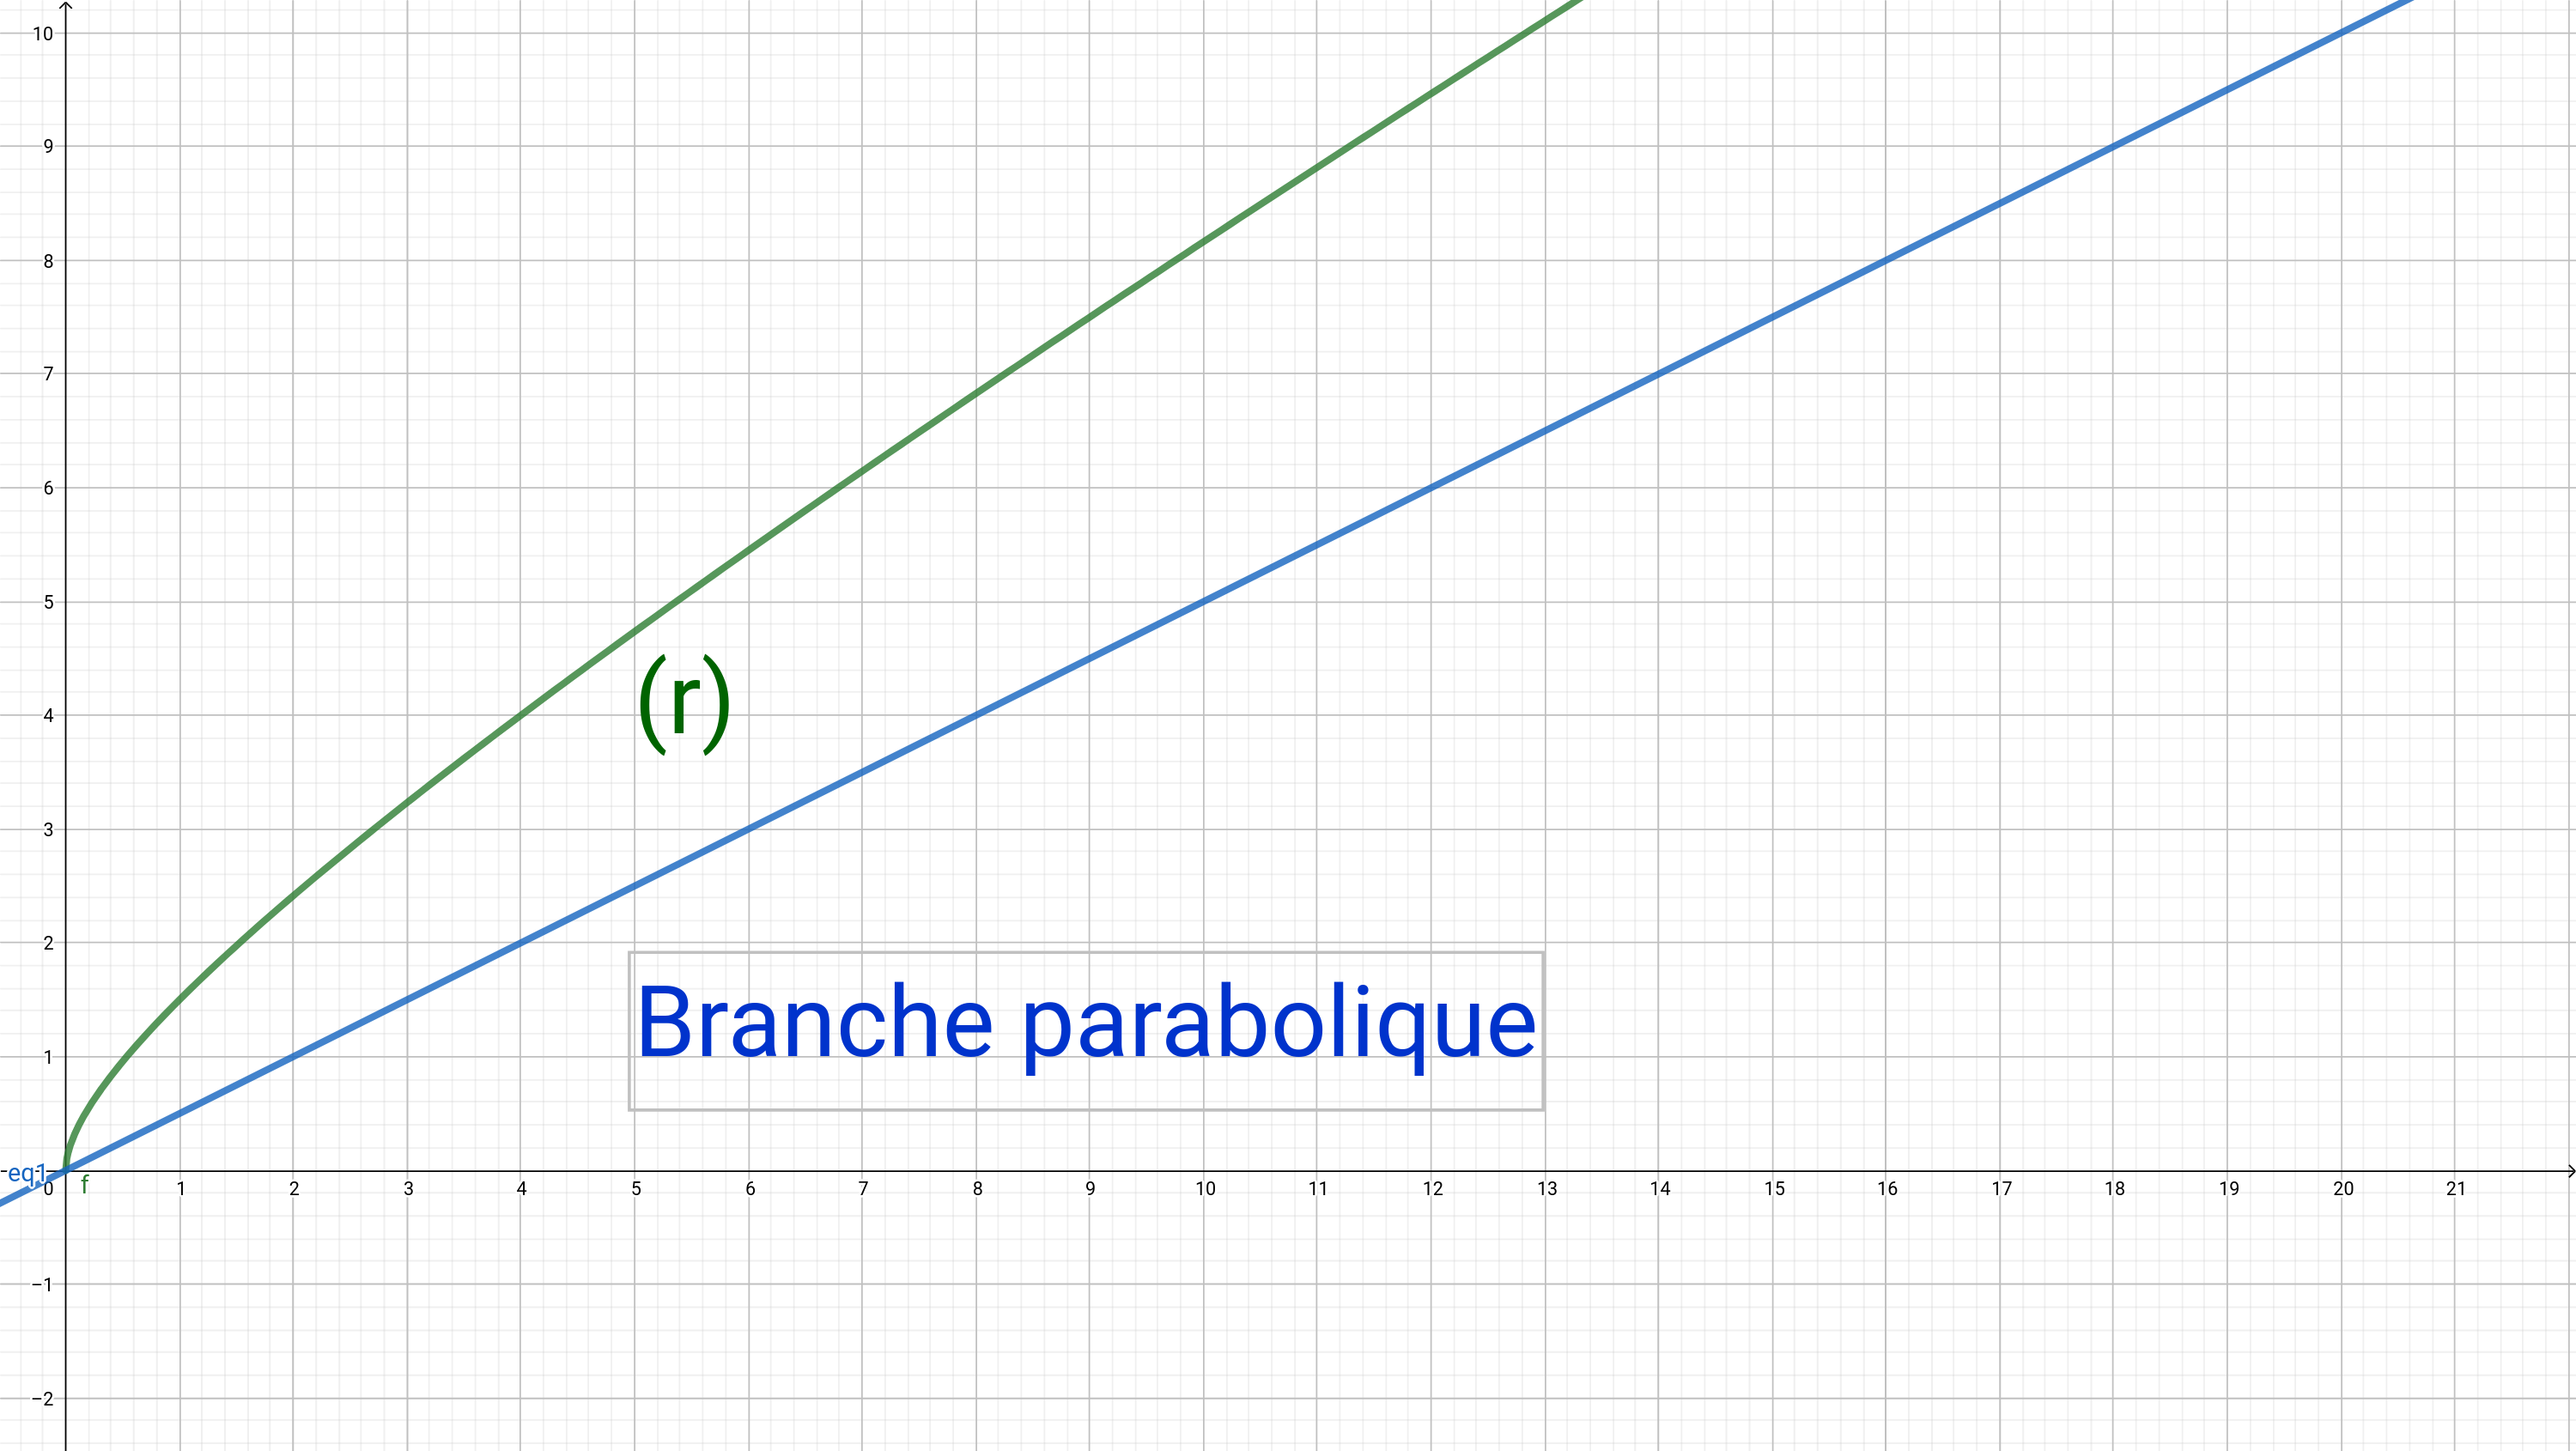
\includegraphics[width=5cm]{images/branche_parabolique.png}
        \end{exampleblock}
\end{frame}

\begin{frame}{Cas n°3$\beta$}
        $\lim_{t\to t_0}\left[y(t)-ax(t)\right]=b$ avec $b\in\mathbb{R}$
        \begin{exampleblock}{Exemple~:}
                \begin{minipage}[b]{5cm}
                        La courbe d'équation $y=\sqrt{t^2-1}+2t$
                        admet une asymptote d'équation $y=3x$
                \end{minipage}
                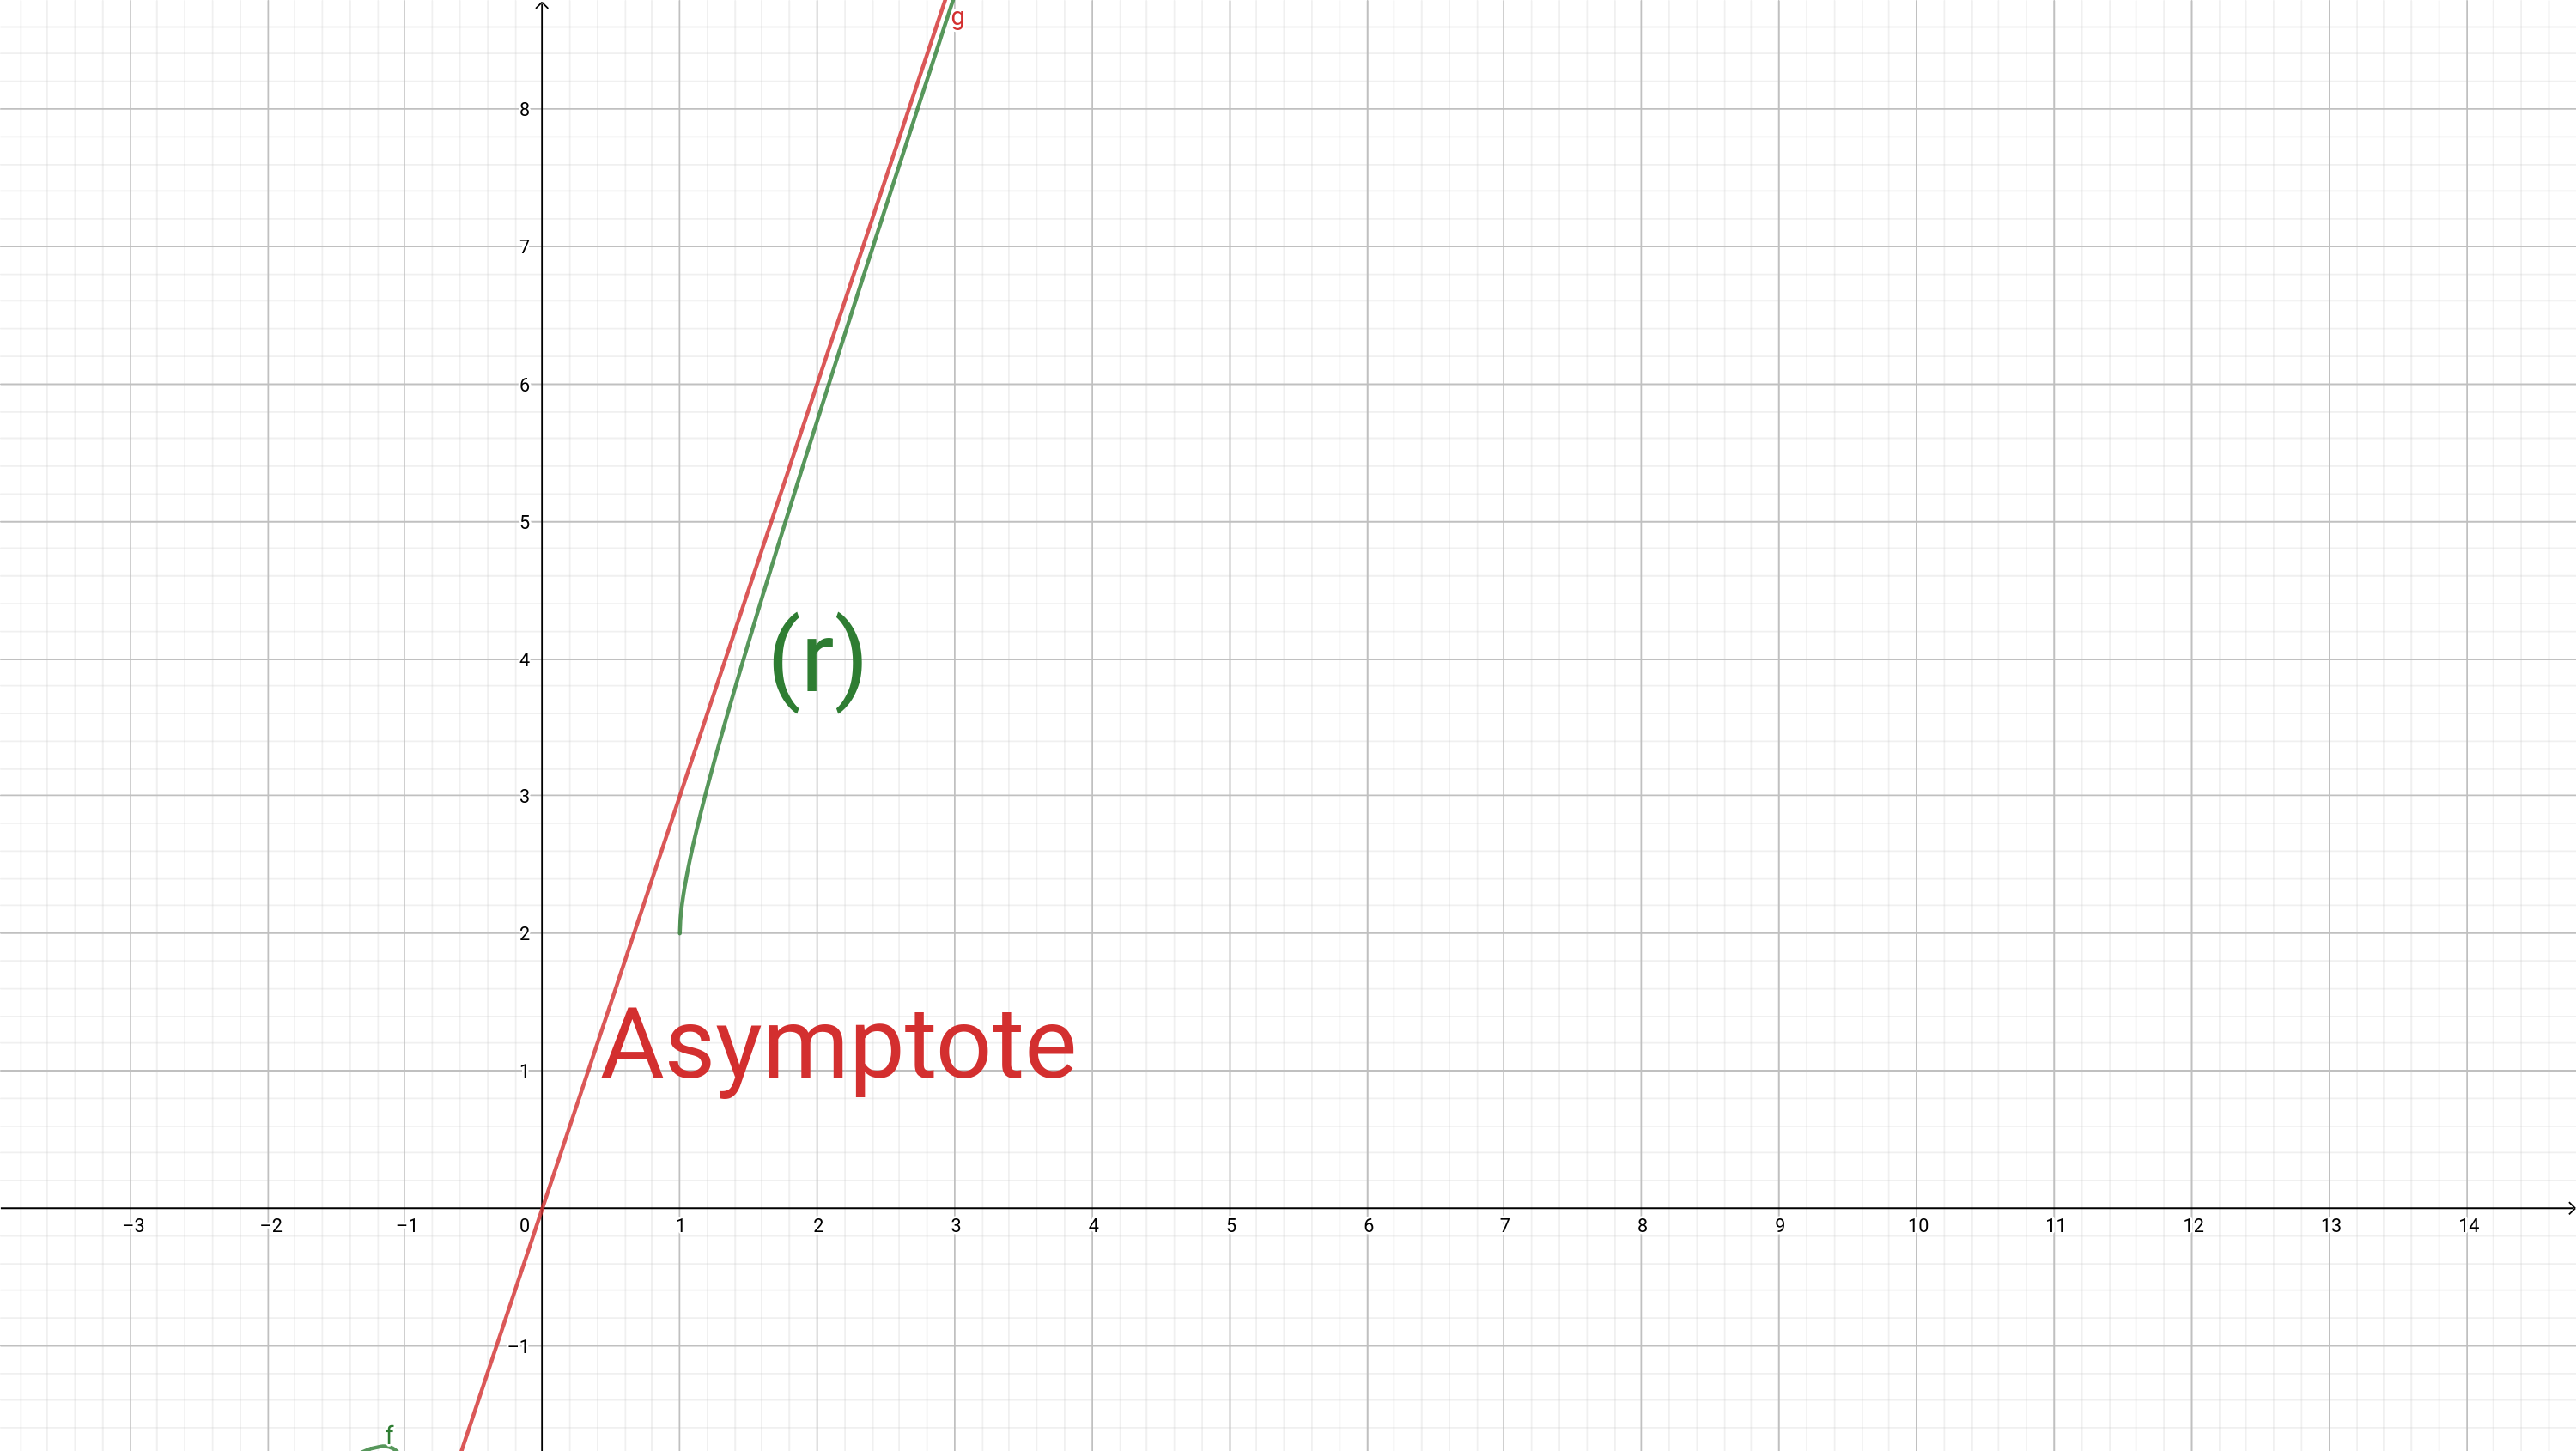
\includegraphics[width=5cm]{images/Asymptote_03.png}
        \end{exampleblock}
\end{frame}

\begin{frame}{}
        \centering Trop facile n'est-ce pas?\\
        \centering Vous pouvez faire les TD des courbes paramétrées en coordonnées cartésiennes.
        Exercices 1 à 3.
\end{frame}

\end{document}
